\documentclass{article}
\usepackage{graphicx}
\usepackage{amsmath}
\usepackage{cite}
\usepackage{color}
\usepackage{enumitem}
\usepackage{hyperref}
\usepackage{natbib}
\usepackage{tabularx}
\usepackage{natbib}
\usepackage{ragged2e}

\title{\textbf{La dis-informazione}}
\author{\texttt{Alessandro Meloni GEPID}}
\date{11/12/2023}

\begin{document}
\maketitle
    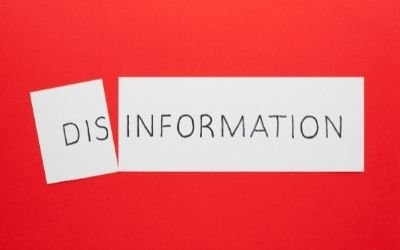
\includegraphics[width = 0.6\linewidth]{Immagini/disinformation.jpeg}
\centering \tableofcontents
\newpage \section{Introduzione}
\flushleft
\begin{justify}
    Questo paper avrà innanzitutto: la finalità di provare a mettere in chiaro cosa si intenda effettivamente per disinformazione; e le varie sfaccettature che questo concetto può assumere.
    Faremo in modo di dare chiarezza in quanto la disinformazione ha un fine negativo e di sviamento, ma anche la sua forma non sempre risulta essere compresa agli occhi dei lettori.
    Partiremo dall'analisi di una survey effettuata da parte dell'Unesco nel 2023, e, pubblicata dal The Guardian come articolo nella loro pagina internet. Questo sarà seguito da un piccolo sondaggio fatto su un campione di X persone, provando a comprendere, almeno in Italia, quale possa essere la tendenza di percezione di questo concetto da parte della popolazione.
    Faremo e spiegheremo dei grafici risultanti dalla survey, così da comprendere quanto possano variare le percezioni sulla disinformazione sulla base di caratteristiche personali. 
    Seguirà successivamente una comparazione con dati relativi alla presenza oggettiva di fake news, così da capire se le percezioni delle persone, poi, coincidono con la frequenza oggettiva del fenomeno all'interno dei vari media.
    In conclusione, vedremo i risultati che ha dato questa ricerca, così da dare dei consigli su come riconoscere informazioni da dis-informazioni, in funzione di creare una maggiore consapevolezza e sicurezza nell'utente/lettore, evitando che questo fenomeno possa davvero portare al fine per cui la notizia viene diffusa.
    
\end{justify}
 
\newpage \section{Il fenomeno della disinformazione}

\flushleft \subsection{Cos'è la disinformazione?}

\flushleft \subsection{Analisi dati}

\flushleft \subsection{L'impatto della disinformazione nella vita delle persone}

\centering
\newpage\section{Riflessioni e conclusioni}

\end{document}